\chapter{Graphically Solving Linear Programs}
\begin{outcome}

\begin{enumerate}
\item[A.] Learn how to plot the feasible region and the objective function.
\item[B.] Identify and compute extreme points of the feasible region.
\item[C.] Find the optimal solution(s) to a linear program graphically.
\item[D.] Classify the type of result of the problem as infeasible, unbounded, unique optimal solution, or infinitely many optimal solutions.
\end{enumerate}
\end{outcome}

Linear Programs (LP's) with two variables can be solved graphically by plotting the feasible region along with the level curves of the objective function.\footnote{Special thanks to Joshua Emmanual and Christopher Griffin for sharing their content to help put this section together. Proper citations and referenes are forthcoming.} We will show that we can find a point in the feasible region that maximizes the objective function using the level curves of the objective function.

We will begin with an easy example that is bounded and investigate the structure of the feasible region.  We will then explore other examples.
\section{Nonempty and Bounded Problem}
Consider the problem
\begin{align*}
\max \quad & 2 X+5 Y \\
\text { s.t. } \quad 
&X+2 Y \leq 16 \\
&5 X+3 Y \leq  45 \\
&X, Y  \geq 0
\end{align*}

We want to start by plotting the \emph{feasible region}, that is, the set points $(X,Y)$ that satisfy all the constraints. 

We can plot this by first plotting the four lines
\begin{itemize}
\item $X+2 Y = 16$
\item $5 X+3 Y = 45$
\item $X = 0$
\item $Y = 0$
\end{itemize}
and then shading in the side of the space cut out by the corresponding inequality.
\begin{center}
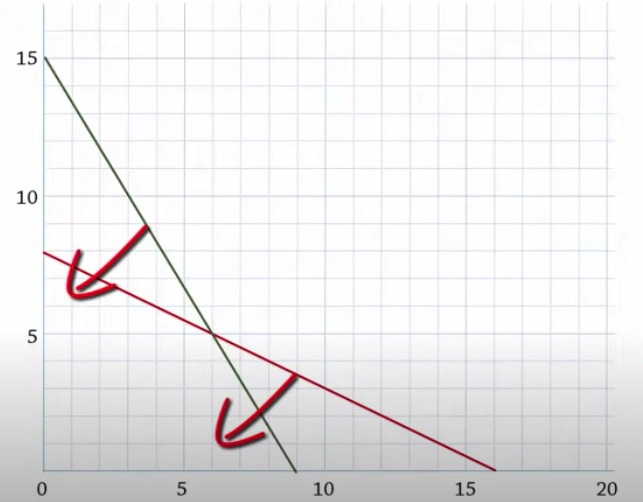
\includegraphics[scale = 0.4]{screenshots/example0-inequalities}
\end{center}

The resulting feasible region can then can be shaded in as the region that satisfies all the inequalties.

\begin{center}
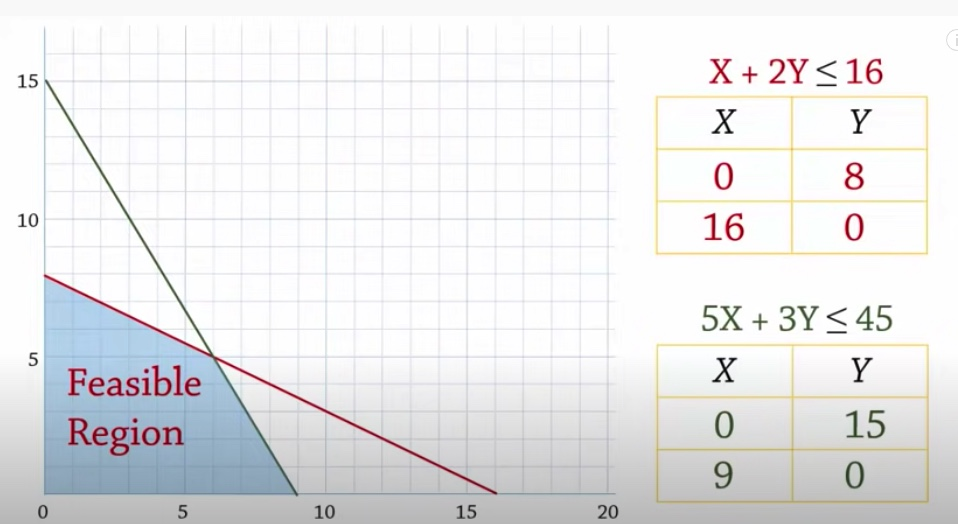
\includegraphics[scale = 0.4]{screenshots/example0-feasible-region}
\end{center}

Notice that the feasible region is nonempty (it has points that satisfy all the inequalities) and also that it is bounded (the feasible points dont continue infinitly in any direction).

We want to identify the \emph{extreme points} (i.e., the corners) of the feasible region. 
Understanding these points will be critical to understanding the optimal solutions of the model.
Notice that all extreme points can be computed by finding the intersection of 2 of the lines.   But!  Not all intersections of any two lines are feasible.  

We will later use the terminology \emph{basic feasible solution} for an extreme point of the feasible region, and \emph{basic solution} as a point that is the intersection of 2 lines, but is actually infeasible (does not satisfy all the constraints).

\begin{center}
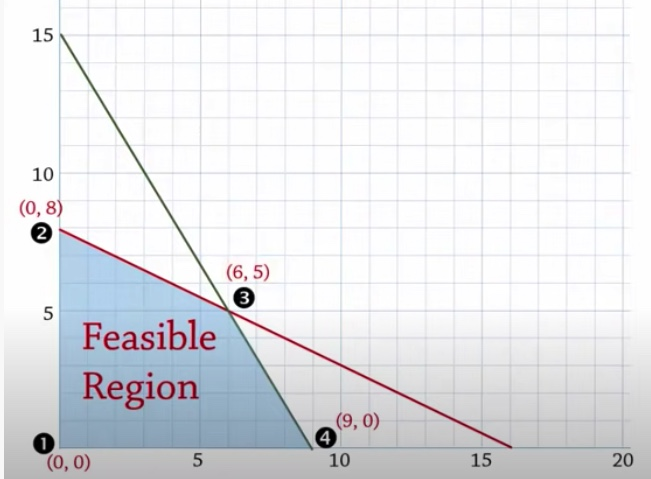
\includegraphics[scale = 0.4]{screenshots/example0-extreme-points}
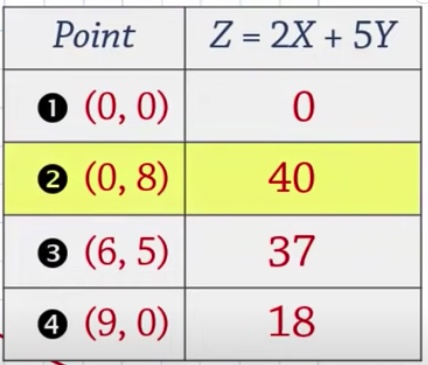
\includegraphics[scale = 0.4]{screenshots/example0-extreme-point-solutions}
\end{center}

\begin{theorem}{Optimal Extreme Point}{optimalextremepoint}
If the feasible region is nonempty and bounded, then there exists an optimal solution at an extreme point of the feasible region.
\end{theorem}

We will explore why this theorem is true, and also what happens when the feasible region does not satisfy the assumtions of either nonempty or bounded.
We illustrate the idea first using the problem from Example \ref{ex:ToyMaker}.

\begin{figure}[H] 
\centering
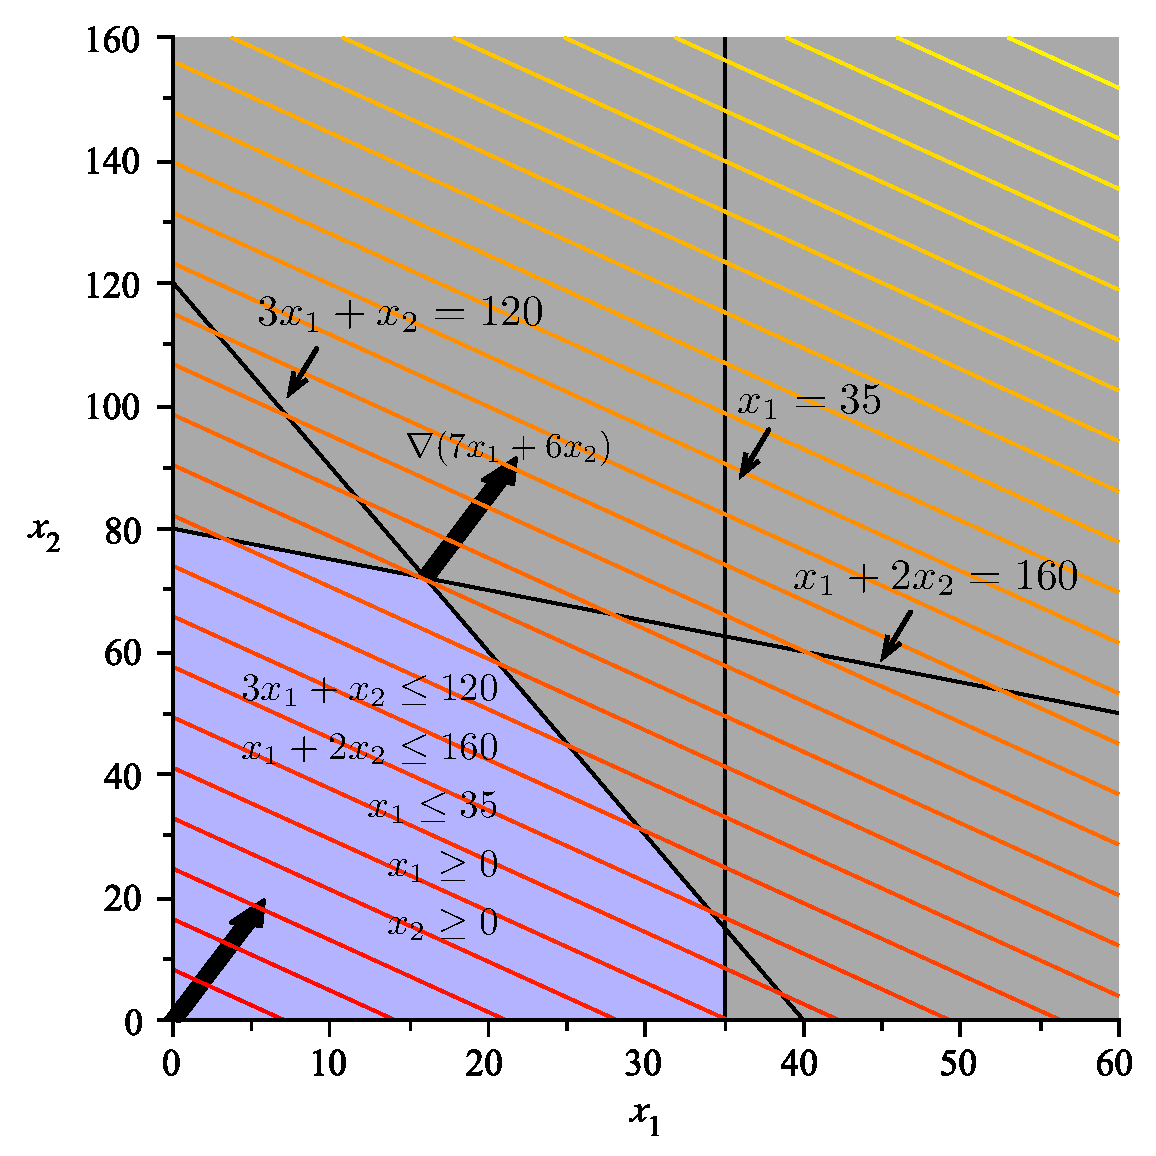
\includegraphics[scale=0.4]{FeasibleRegion.pdf}
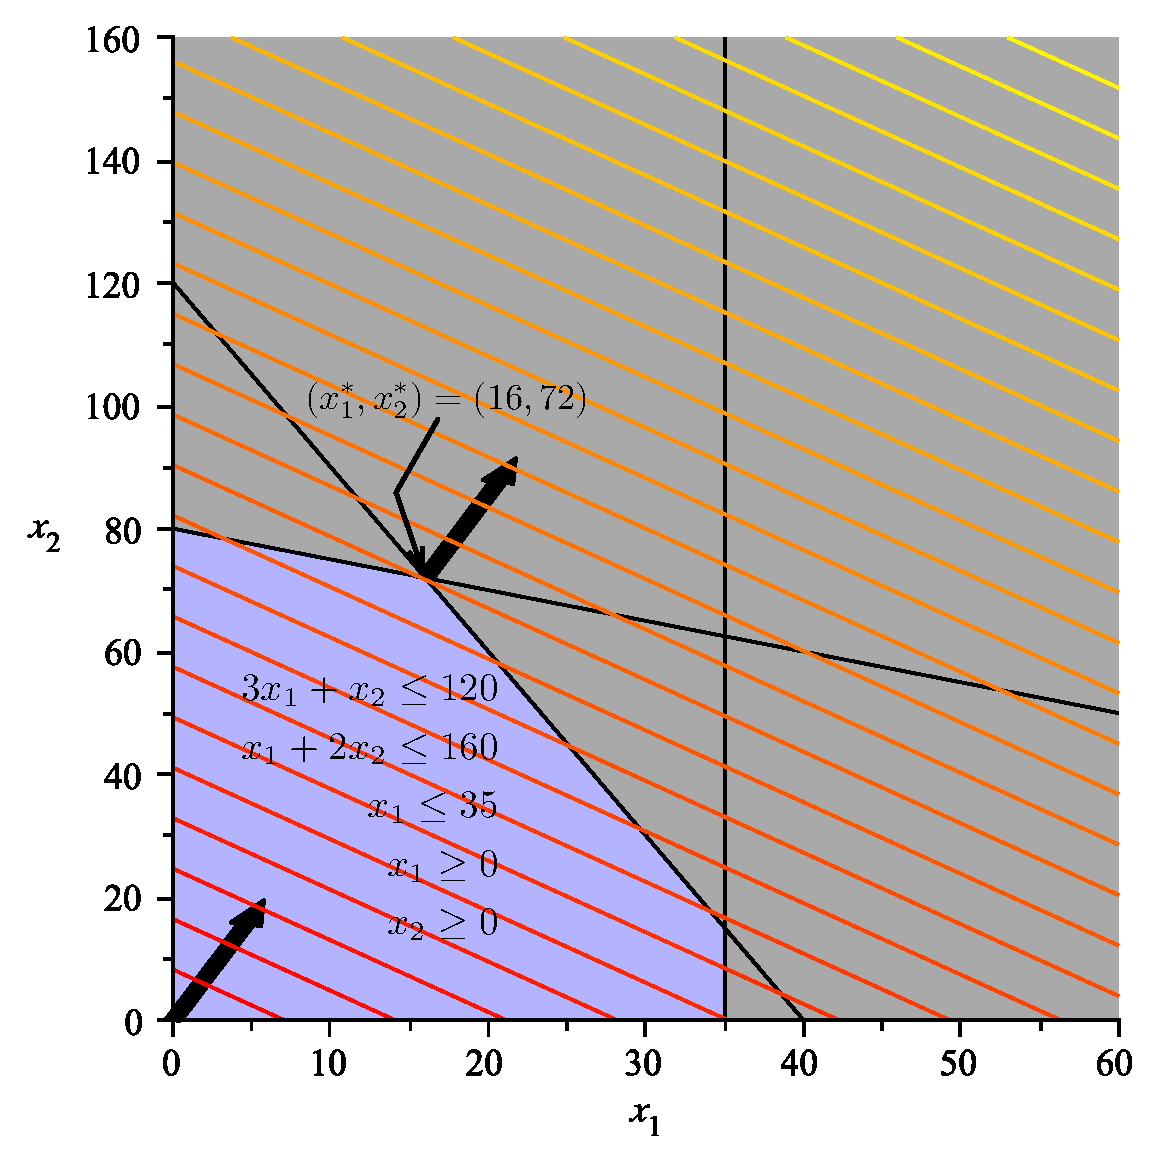
\includegraphics[scale=0.4]{FeasibleRegionWithMax.pdf}
\caption{Feasible Region and Level Curves of the Objective Function: The shaded region in the plot is the feasible region and represents the intersection of the five inequalities constraining the values of $x_1$ and $x_2$. On the right, we see the optimal solution is the ``last'' point in the feasible region that intersects a level set as we move in the direction of increasing profit.}
\label{fig:ToyExampleFeasibleRegion}
\end{figure}

\begin{example}{Continuation of Example \ref{ex:ToyMaker}}{}Let's continue the example of the Toy Maker begin in Example \ref{ex:ToyMaker}.  Solve this problem graphically.
\end{example}
\begin{solution} To solve the linear programming problem graphically, begin by drawing the feasible region. This is shown in the blue shaded region of Figure \ref{fig:ToyExampleFeasibleRegion}. 


After plotting the feasible region, the next step is to plot the level curves of the objective function. In our problem, the level sets will have the form:
\begin{displaymath}
7x_1 + 6x_2 = c \implies x_2 = \frac{-7}{6}x_1 + \frac{c}{6}
\end{displaymath}
This is a set of parallel lines with slope $-7/6$ and intercept $c/6$ where $c$ can be varied as needed. The level curves for various values of $c$ are parallel lines. In Figure \ref{fig:ToyExampleFeasibleRegion} they are shown in colors ranging from red to yellow depending upon the value of $c$. Larger values of $c$ are more yellow. 

To solve the linear programming problem, follow the level sets along the gradient (shown as the black arrow) until the last level set (line) intersects the feasible region. If you are doing this by hand, you can draw a single line of the form $7x_1 + 6x_2 = c$ and then simply draw parallel lines in the direction of the gradient $(7,6)$. At some point, these lines will fail to intersect the feasible region. The last line to intersect the feasible region will do so at a point that maximizes the profit. In this case, the point that maximizes $z(x_1,x_2) = 7x_1 + 6x_2$, subject to the constraints given, is $(x_1^*, x_2^*) = (16,72)$. 
\newpage
Note the point of optimality $(x_1^*, x_2^*) = (16,72)$ is at a corner of the feasible region. This corner is formed by the intersection of the two lines: $3x_1 + x_2 = 120$ and $x_1 + 2x_2 = 160$. In this case, the constraints 
\begin{gather*}
3x_1 + x_2 \leq 120\\
x_1 + 2x_2 \leq 160
\end{gather*}
are both \textit{binding}, while the other constraints are non-binding. In general, we will see that when an optimal solution to a linear programming problem exists, it will always be at the intersection of several binding constraints; that is, it will occur at a corner of a higher-dimensional polyhedron.  
\end{solution}

We can now define an algorithm for identifying the solution to a linear programing problem in two variables with a \textit{bounded} feasible region (see Algorithm \ref{alg:GraphLPBoundedUniqueSoln}): 
\begin{algorithm}
\caption{Algorithm for Solving a Two Variable Linear Programming Problem Graphically--Bounded Feasible Region, Unique Solution Case}
\label{alg:GraphLPBoundedUniqueSoln}
\begin{center}
\begin{minipage}[t]{\textwidth-1em}
\underline{\textbf{Algorithm for Solving a Linear Programming Problem Graphically}}\\
\textit{Bounded Feasible Region, Unique Solution}
\begin{enumerate*}
\item Plot the feasible region defined by the constraints.
\item Plot the level sets of the objective function.
\item For a maximization problem, identify the level set corresponding the greatest (least, for minimization) objective function value that intersects the feasible region. This point will be at a corner. 
\item The point on the corner intersecting the greatest (least) level set is a solution to the linear programming problem.  
\end{enumerate*}
\end{minipage}
\end{center}
\end{algorithm}

The example linear programming problem presented in the previous section has a single optimal solution. In general, the following outcomes can occur in solving a linear programming problem: 
\begin{enumerate*}
\item The linear programming problem has a unique solution. (We've already seen this.)
\item There are infinitely many alternative optimal solutions.
\item There is no solution and the problem's objective function can grow to positive infinity for maximization problems (or negative infinity for minimization problems). 
\item There is no solution to the problem at all. 
\end{enumerate*}

Case 3 above can only occur when the feasible region is unbounded; that is, it cannot be surrounded by a ball with finite radius. We will illustrate each of these possible outcomes in the next four sections. We will prove that this is true in a later chapter.



\section{Infinitely Many Optimal Solutions}
It can happen that there is more than one solution.  In fact, in this case, there are infinitly many optimal solutions.  
We'll study a specific linear programming problem with an infinite number of solutions by modifying the objective function in Example \ref{ex:ToyMaker}. 
\begin{example}{Toy Maker Alternative Solutions}{ex:ToyMakerAltOptSoln}
Suppose the toy maker in Example \ref{ex:ToyMaker} finds that it can sell planes for a profit of $\$18$ each instead of $\$7$ each. The new linear programming problem becomes:
\begin{equation}
\left\{
\begin{aligned}
\max\;\;& z(x_1,x_2) = 18x_1 + 6x_2\\
s.t.\;\;&  3x_1 + x_2 \leq 120\\
& x_1 + 2x_2 \leq 160\\
& x_1 \leq 35\\
& x_1 \geq 0\\
& x_2 \geq 0
\end{aligned}
\right.
\label{eqn:ToyMakerAltOptSoln}
\end{equation}
\end{example}

\begin{solution}
Applying our graphical method for finding optimal solutions to linear programming problems yields the plot shown in Figure \ref{fig:ToyMakerAltOptSoln}. The level curves for the function $z(x_1,x_2) = 18x_1 + 6x_2$ are \textit{parallel} to one face of the polygon boundary of the feasible region. Hence, as we move further up and to the right in the direction of the gradient (corresponding to larger and larger values of $z(x_1, x_2)$) we see that there is not \textit{one} point on the boundary of the feasible region that intersects that level set with greatest value, but instead a side of the polygon boundary described by the line $3x_1 + x_2 = 120$ where $x_1 \in [16, 35]$. Let:
\begin{displaymath}
S = \{(x_1,x_2) | 3x_1 + x_2 \leq 120,\,x_1 + 2x_2 \leq 160,\,x_1 \leq 35,\,x_1,x_2 \geq 0\}
\end{displaymath} 
that is, $S$ is the feasible region of the problem. Then for any value of $x_1^* \in [16,35]$ and any value $x_2^*$ so that  $3x_1^* + x_2^* = 120$, we will have $z(x_1^*, x_2^*) \geq z(x_1, x_2)$ for all $(x_1,x_2) \in S$. Since there are infinitely many values that $x_1$ and $x_2$  may take on, we see this problem has an infinite number of alternative optimal solutions.
\begin{figure}[H]
\centering
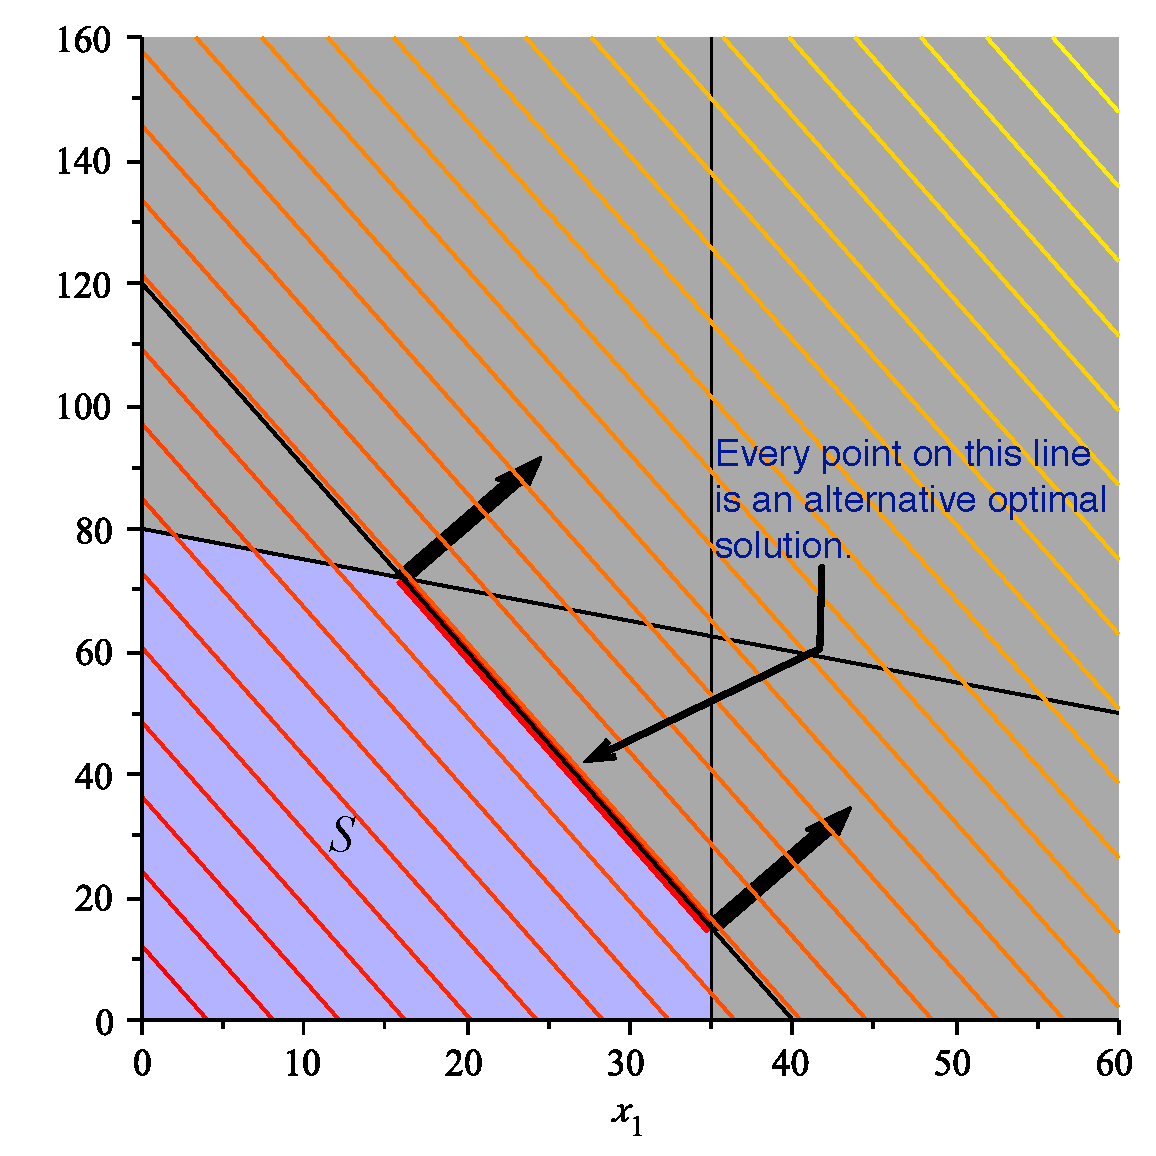
\includegraphics[scale=0.4]{AltOptSolns.pdf}
\caption{An example of infinitely many alternative optimal solutions in a linear programming problem. The level curves for $z(x_1,x_2) = 18x_1 + 6x_2$ are \textit{parallel} to one face of the polygon boundary of the feasible region. Moreover, this side contains the points of greatest value for $z(x_1,x_2)$ inside the feasible region. Any combination of $(x_1,x_2)$ on the line $3x_1 + x_2 = 120$ for $x_1 \in [16, 35]$ will provide the largest possible value $z(x_1,x_2)$ can take in the feasible region $S$.}
\label{fig:ToyMakerAltOptSoln}
\end{figure}
%\label{ex:ToyMakerAltOptSoln}
\end{solution}






\begin{exercise}{}{} Use the graphical method for solving linear programming problems to solve the linear programming problem you defined in Exercise \ref{exer:ChemicalPlant}.
\end{exercise}



Based on the example in this section, we can modify our algorithm for finding the solution to a linear programming problem graphically to deal with situations with an infinite set of alternative optimal solutions (see Algorithm \ref{alg:GraphLPBounded}):
\begin{algorithm}[H]
\caption{Algorithm for Solving a Two Variable Linear Programming Problem Graphically--Bounded Feasible Region Case}
\label{alg:GraphLPBounded}
\begin{center}
\begin{minipage}[t]{\textwidth-1em}
\underline{\textbf{Algorithm for Solving a Linear Programming Problem Graphically}}\\
\textit{Bounded Feasible Region}
\begin{enumerate*}
\item Plot the feasible region defined by the constraints.
\item Plot the level sets of the objective function.
\item For a maximization problem, identify the level set corresponding the greatest (least, for minimization) objective function value that intersects the feasible region. This point will be at a corner. 
\item The point on the corner intersecting the greatest (least) level set is a solution to the linear programming problem. 
\item \textbf{If the level set corresponding to the greatest (least) objective function value is parallel to a side of the polygon boundary next to the corner identified, then there are infinitely many alternative optimal solutions and any point on this side may be chosen as an optimal solution.} 
\end{enumerate*}
\end{minipage}
\end{center}
\end{algorithm}

\begin{exercise}{}{} Modify the linear programming problem from Exercise \ref{exer:ChemicalPlant} to obtain a linear programming problem with an infinite number of alternative optimal solutions. Solve the new problem and obtain a description for the set of alternative optimal solutions. [Hint: Just as in the example, $x_1$ will be bound between two value corresponding to a side of the polygon. Find those values and the constraint that is binding. This will provide you with a description of the form for any $x_1^* \in [a,b]$ and $x_2^*$ is chosen so that $cx_1^* + dx_2^* = v$, the point $(x_1^*, x_2^*)$ is an alternative optimal solution to the problem. Now you fill in values for $a$, $b$, $c$, $d$ and $v$.]
\end{exercise}

\section{Problems with No Solution} Recall for \textit{any} mathematical programming problem, the feasible set or region is simply a subset of $\mathbb{R}^n$. If this region is empty, then there is no solution to the mathematical programming problem and the problem is said to be \textit{over constrained}. In this case, we say that the problem is \emph{infeasible}.  We illustrate this case for linear programming problems with the following example.
\begin{example}{Infeasible Problem}
 Consider the following linear programming problem:
\begin{equation}
\left\{
\begin{aligned}
\max\;\;& z(x_1,x_2) = 3x_1 + 2x_2\\
s.t.\;\;&  \frac{1}{40}x_1 + \frac{1}{60}x_2 \leq 1\\
& \frac{1}{50}x_1 + \frac{1}{50}x_2 \leq 1\\
& x_1 \geq 30\\
& x_2 \geq 20
\end{aligned}
\right.
\label{eqn:LPInfeasible}
\end{equation}
\end{example}
\begin{solution}
The level sets of the objective and the constraints are shown in Figure \ref{fig:LPInfeasible}. 
\begin{figure}[H]
\centering
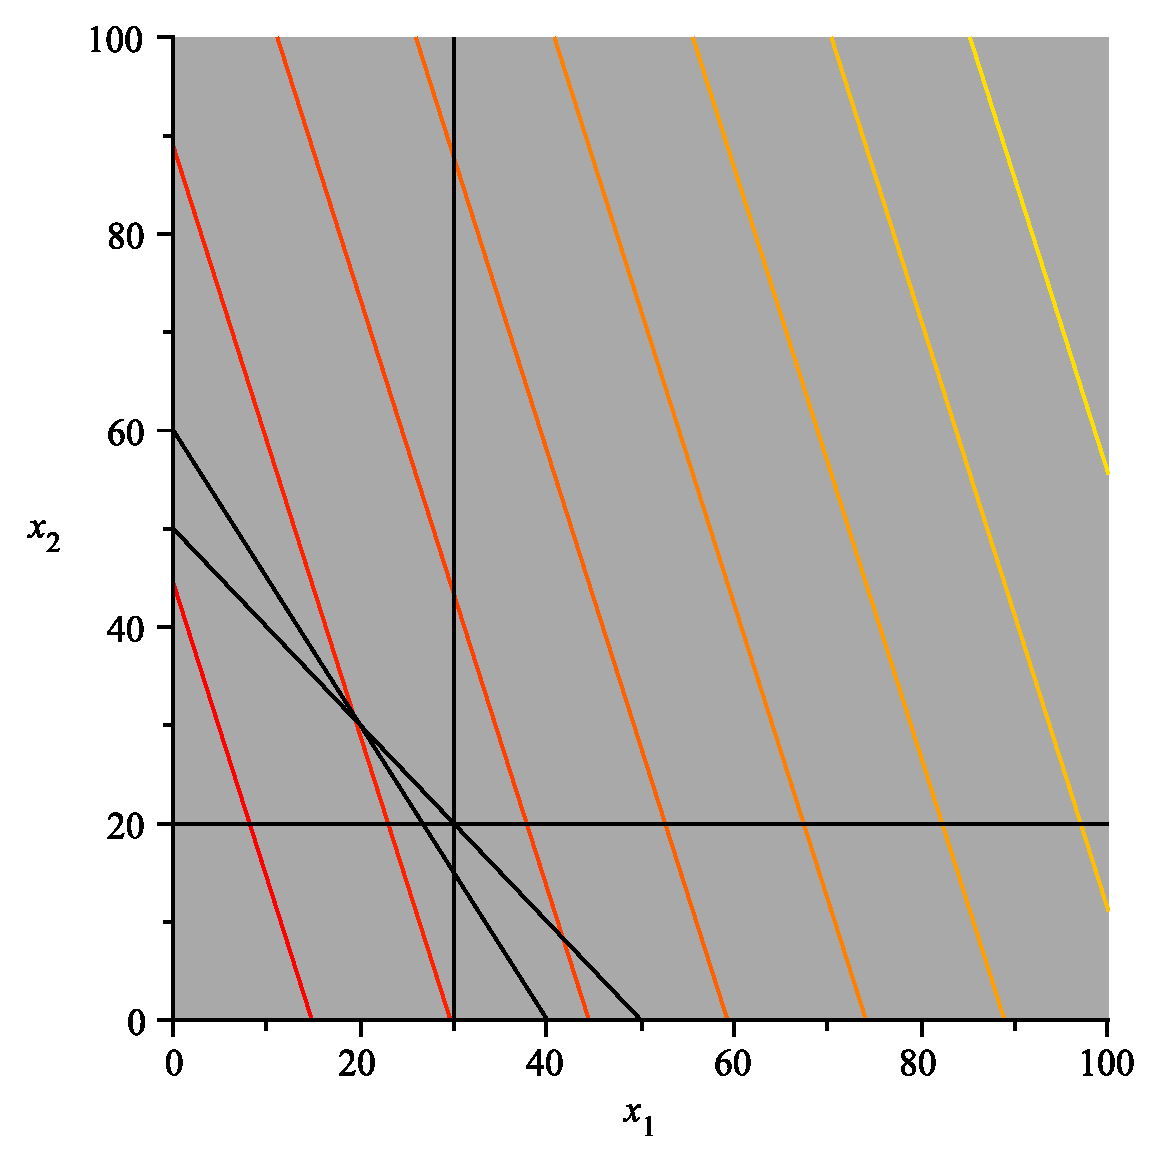
\includegraphics[scale=0.4]{LPNoSoln.pdf}
\caption{A Linear Programming Problem with no solution. The feasible region of the linear programming problem is empty; that is, there are no values for $x_1$ and $x_2$ that can simultaneously satisfy all the constraints. Thus, no solution exists.}
\label{fig:LPInfeasible}
\end{figure}

The fact that the feasible region is empty is shown by the fact that in Figure \ref{fig:LPInfeasible} there is no blue region--i.e., all the regions are gray indicating that the constraints are not satisfiable.
\label{ex:LPNoSoln}
\end{solution} 
Based on this example, we can modify our previous algorithm for finding the solution to linear programming problems graphically (see Algorithm \ref{alg:GraphLPBoundedEmpty}):
\begin{algorithm}[H]
\caption{Algorithm for Solving a Two Variable Linear Programming Problem Graphically--Bounded Feasible Region Case}
\label{alg:GraphLPBoundedEmpty}
\begin{center}
\begin{minipage}[t]{\textwidth-1em}
\underline{\textbf{Algorithm for Solving a Linear Programming Problem Graphically}}\\
\textit{Bounded Feasible Region}
\begin{enumerate*}
\item Plot the feasible region defined by the constraints.
\item \textbf{If the feasible region is empty, then no solution exists.}
\item Plot the level sets of the objective function.
\item For a maximization problem, identify the level set corresponding the greatest (least, for minimization) objective function value that intersects the feasible region. This point will be at a corner. 
\item The point on the corner intersecting the greatest (least) level set is a solution to the linear programming problem. 
\item \textbf{If the level set corresponding to the greatest (least) objective function value is parallel to a side of the polygon boundary next to the corner identified, then there are infinitely many alternative optimal solutions and any point on this side may be chosen as an optimal solution.} 
\end{enumerate*}
\end{minipage}
\end{center}
\end{algorithm}

\section{Problems with Unbounded Feasible Regions}

Consider the problem

\begin{align*}
\min \quad & Z =5 X+7 Y  \\ 
\text { s.t. } \quad & X+3 Y \geq 6 \\ 
&5 X+ 2 Y \geq 10 \\ 
&Y  \leq 4 \\ 
&X, Y  \geq 0 
\end{align*}

\begin{center}
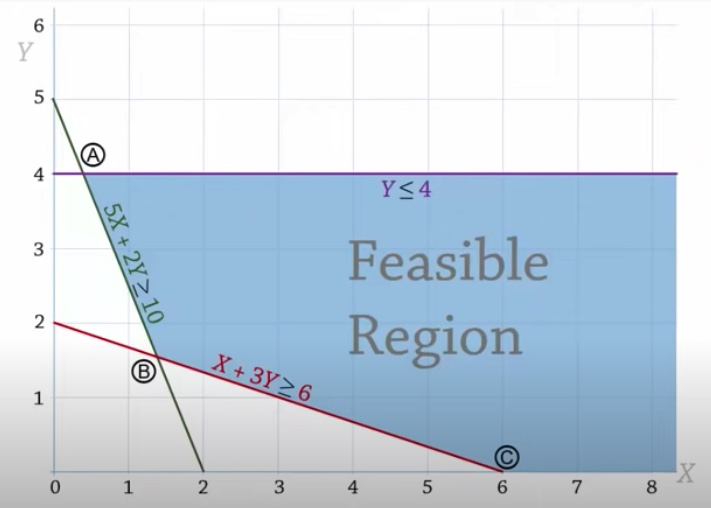
\includegraphics[scale = 0.4]{screenshots/example1-feasible-region}
\end{center}

As you can see, the feasible region is \emph{unbounded}.  In particular, from any point in the feasible region, one can always find another feasible point by increasing the $X$ coordinate (i.e., move to the right in the picture).   However, this does not necessarily mean that the optimization problem is unbounded.

Indeed, the optimal solution is at the B, the extreme point in the lower left hand corner.

\todo[inline]{To do: add contours to plot to show extreme point is the optimal solution.}

\begin{center}
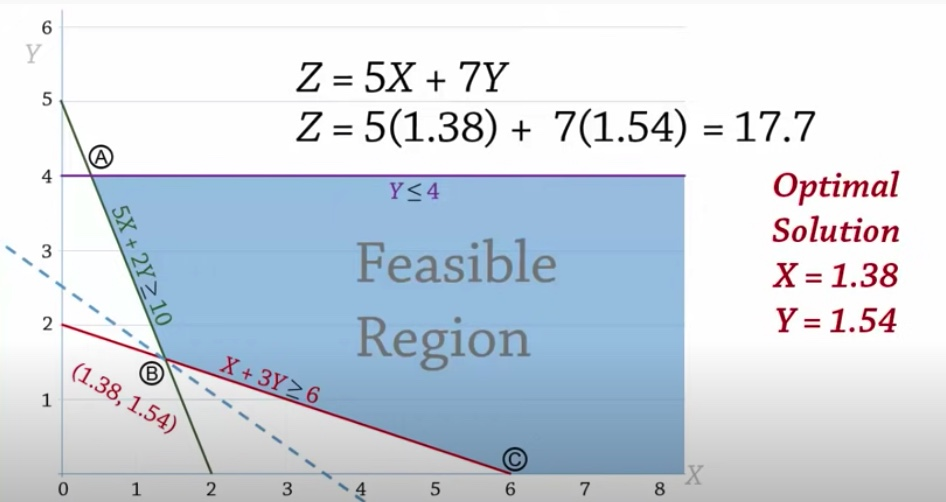
\includegraphics[scale = 0.4]{screenshots/example1-optimal-solution}
\end{center}


Consider however, if we consider a different problem where we try to maximize the objective
\begin{align*}
\max \quad & Z = 5X + 7Y\\ 
\text { s.t. } \quad & X+3 Y \geq 6 \\ 
&5 X+ 2 Y \geq 10 \\ 
&Y  \leq 4 \\ 
&X, Y  \geq 0 
\end{align*}

\begin{solution}
This optimization problem is unbounded!  For example, notice that the point $(X,Y) = (n,0)$ is feasible for all $n=1,2,3,\dots,$.   Then the objective function $Z = 5n + 0$ follows the sequence $5, 10, 15, \dots,$, which diverges to infinity.   
\end{solution}


Again, we'll tackle the issue of linear programming problems with unbounded feasible regions by illustrating the possible outcomes using examples.

\begin{example}{}{} Consider the linear programming problem below:
\begin{equation}
\left\{
\begin{aligned}
\max\;\;& z(x_1,x_2) = 2x_1 - x_2\\
s.t.\;\;& x_1 - x_2 \leq 1\\
& 2x_1 + x_2 \geq 6\\
&x_1,x_2 \geq 0
\end{aligned}
\right.
\label{eqn:LPUnboundFeasibleRegion1}
\end{equation}
\end{example}
\begin{solution}
The feasible region and level curves of the objective function are shown in Figure \ref{fig:LPUnboundFeasibleRegion1}. 
\begin{figure}[H]%[htbp]
\centering
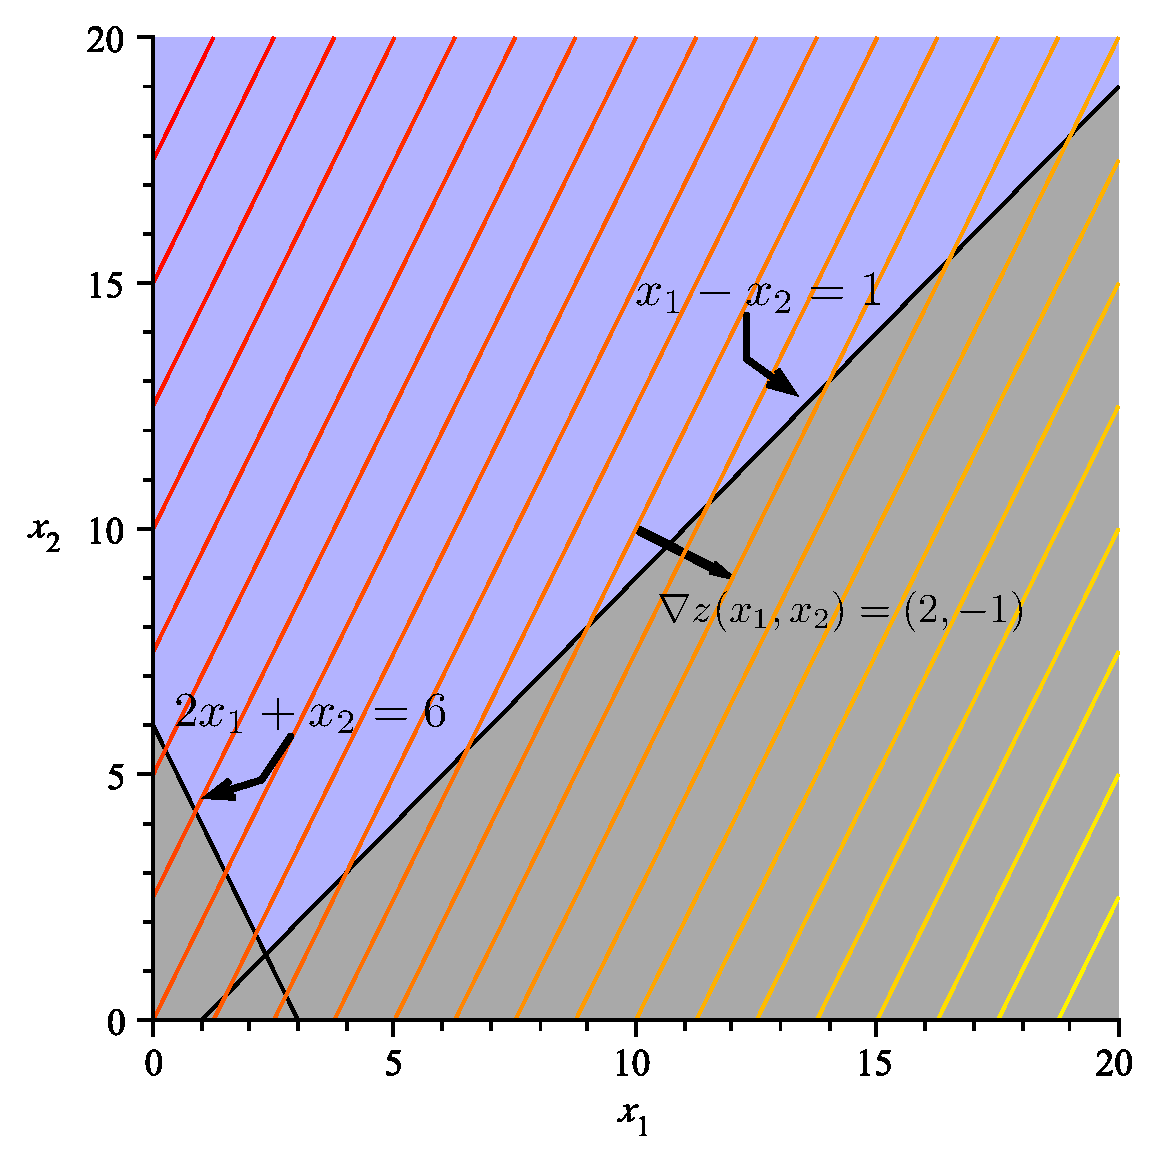
\includegraphics[scale=0.4]{UnboundedFeasibleRegion.pdf}
\caption{A Linear Programming Problem with Unbounded Feasible Region: Note that we can continue to make level curves of $z(x_1,x_2)$ corresponding to larger and larger values as we move down and to the right. These curves will continue to intersect the feasible region for any value of $v = z(x_1,x_2)$ we choose. Thus, we can make $z(x_1,x_2)$ as large as we want and still find a point in the feasible region that will provide this value. Hence, the optimal value of $z(x_1,x_2)$ subject to the constraints $+\infty$. That is, the problem is unbounded.}
\label{fig:LPUnboundFeasibleRegion1}
\end{figure}
The feasible region in Figure \ref{fig:LPUnboundFeasibleRegion1} is clearly unbounded since it stretches upward along the $x_2$ axis infinitely far and also stretches rightward along the $x_1$ axis infinitely far, bounded below by the line $x_1-x_2 = 1$. There is no way to enclose this region by a disk of finite radius, hence the feasible region is not bounded. 

We can draw more level curves of $z(x_1,x_2)$  in the direction of increase (down and to the right) as long as we wish. There will always be an intersection point with the feasible region because it is infinite. That is, these curves will continue to intersect the feasible region for any value of $v = z(x_1,x_2)$ we choose. Thus, we can make $z(x_1,x_2)$ as large as we want and still find a point in the feasible region that will provide this value. Hence, the largest value $z(x_1,x_2)$ can take when $(x_1,x_2)$ are in the feasible region is $+\infty$. That is, the problem is unbounded.
\label{ex:LPUnboundFeasibleRegion1}
\end{solution}

Just because a linear programming problem has an unbounded feasible region does not imply that there is not a finite solution. We illustrate this case by modifying example \ref{ex:LPUnboundFeasibleRegion1}. 

\begin{example}{Continuation of Example \ref{ex:LPUnboundFeasibleRegion1}}{ex:LPUnboundFeasibleRegion2}
Consider the linear programming problem from Example \ref{ex:LPUnboundFeasibleRegion1} with the new objective function: $z(x_1,x_2) = (1/2)x_1 - x_2$. Then we have the new problem:
\begin{equation}
\left\{
\begin{aligned}
\max\;\;& z(x_1,x_2) =\frac{1}{2}x_1 - x_2\\
s.t.\;\;& x_1 - x_2 \leq 1\\
& 2x_1 + x_2 \geq 6\\
&x_1,x_2 \geq 0
\end{aligned}
\right.
\label{eqn:LPUnboundFeasibleRegion2}
\end{equation}
\end{example}
\begin{solution}
The feasible region, level sets of $z(x_1,x_2)$ and gradients are shown in Figure \ref{fig:LPUnboundFeasibleRegion2}. In this case note, that the direction of increase of the objective function is \textit{away} from the direction in which the feasible region is unbounded (i.e., downward). As a result, the point in the feasible region with the largest $z(x_1,x_2)$ value is $(7/3,4/3)$. Again this is a vertex: the binding constraints are $x_1 - x_2 = 1$ and $2x_1 + x_2 = 6$ and the solution occurs at the point these two lines intersect.
\begin{figure}[H]%[htbp]
\centering
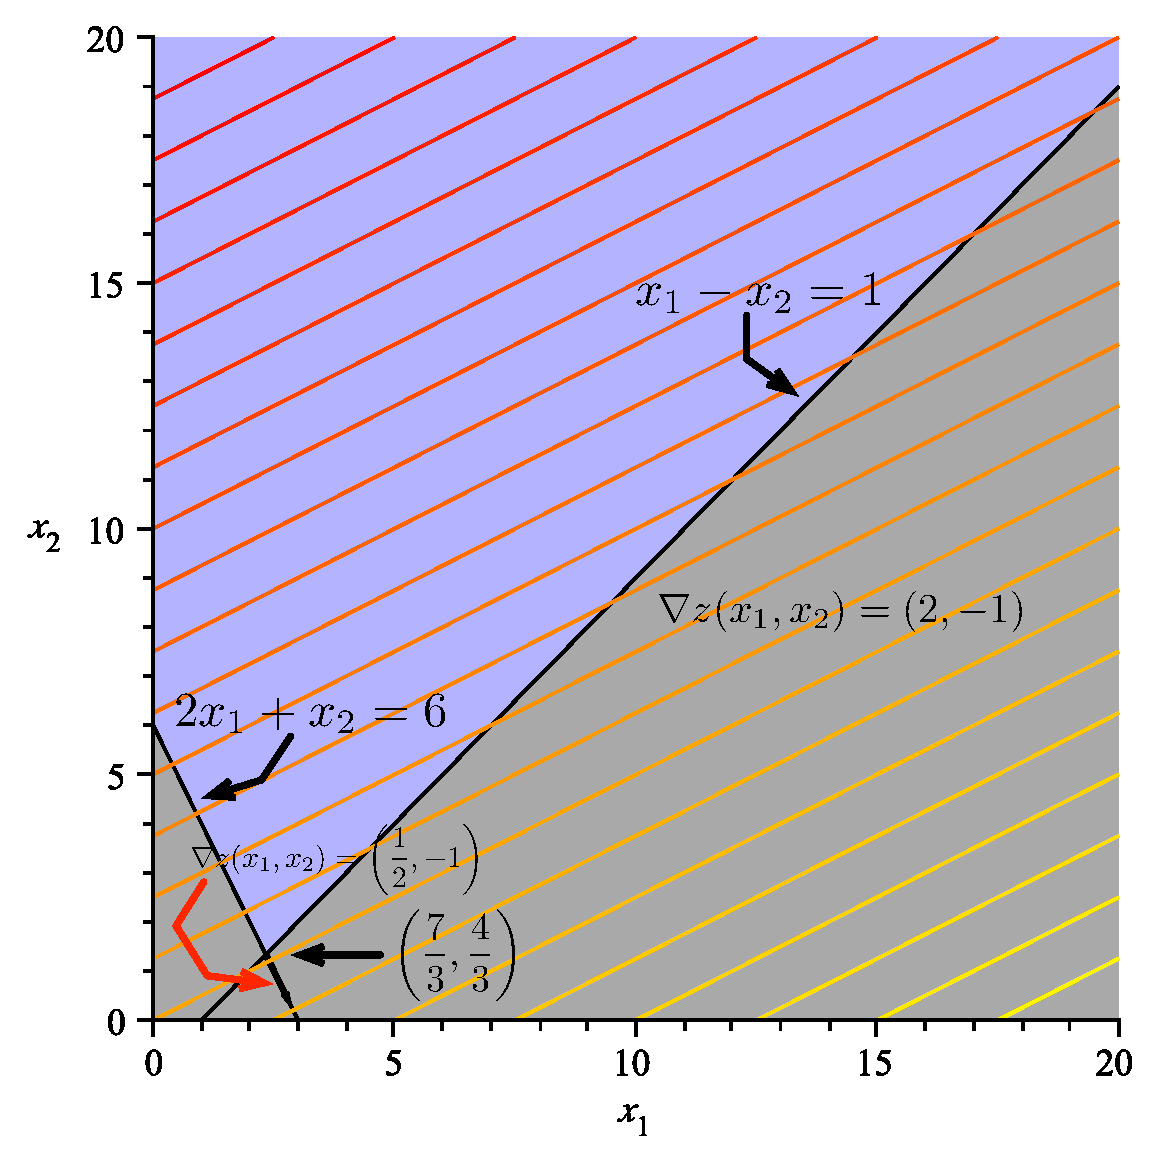
\includegraphics[scale=0.4]{UnboundedFeasibleRegionFiniteSolution.pdf}
\caption{A Linear Programming Problem with Unbounded Feasible Region and Finite Solution: In this problem, the level curves of $z(x_1,x_2)$ increase in a more ``southernly'' direction that in Example \ref{ex:LPUnboundFeasibleRegion2}--that is, \textit{away} from the direction in which the feasible region increases without bound. The point in the feasible region with largest $z(x_1,x_2)$ value is $(7/3,4/3)$. Note again, this is a vertex.}
\label{fig:LPUnboundFeasibleRegion2}
\end{figure}
\label{ex:LPUnboundFeasibleRegion2}
\end{solution}
Based on these two examples, we can modify our algorithm for graphically solving a two variable linear programming problems to deal with the case when the feasible region is unbounded.
\begin{algorithm}
\caption{Algorithm for Solving a Linear Programming Problem Graphically--Bounded and Unbounded Case}
\label{alg:GraphLPAlmostGeneral}
\begin{center}
\begin{minipage}[t]{\textwidth-1em}
\underline{\textbf{Algorithm for Solving a Two Variable Linear Programming Problem Graphically}}
\begin{enumerate*}
\item Plot the feasible region defined by the constraints.
\item If the feasible region is empty, then no solution exists.
\item If the feasible region is unbounded goto Line 8. Otherwise, Goto Line 4.
\item Plot the level sets of the objective function.
\item For a maximization problem, identify the level set corresponding the greatest (least, for minimization) objective function value that intersects the feasible region. This point will be at a corner. 
\item The point on the corner intersecting the greatest (least) level set is a solution to the linear programming problem. 
\item \textbf{If the level set corresponding to the greatest (least) objective function value is parallel to a side of the polygon boundary next to the corner identified, then there are infinitely many alternative optimal solutions and any point on this side may be chosen as an optimal solution.} 
\item (The feasible region is unbounded): Plot the level sets of the objective function.
\item If the level sets intersect the feasible region at larger and larger (smaller and smaller for a minimization problem), then the problem is unbounded and the solution is $+\infty$ ($-\infty$ for minimization problems). 
\item Otherwise, identify the level set corresponding the greatest (least, for minimization) objective function value that intersects the feasible region. This point will be at a corner. 
\item The point on the corner intersecting the greatest (least) level set is a solution to the linear programming problem. 
\textbf{If the level set corresponding to the greatest (least) objective function value is parallel to a side of the polygon boundary next to the corner identified, then there are infinitely many alternative optimal solutions and any point on this side may be chosen as an optimal solution.} 
\end{enumerate*}
\end{minipage}
\end{center}
\end{algorithm}

\begin{exercise}{}{} Does the following problem have a bounded solution? Why?
\begin{equation}
\left\{
\begin{aligned}
\boldsymbol{\min}\;\;& z(x_1,x_2) = 2x_1 - x_2\\
s.t.\;\;& x_1 - x_2 \leq 1\\
& 2x_1 + x_2 \geq 6\\
&x_1,x_2 \geq 0
\end{aligned}
\right.
\end{equation}
[Hint: Use Figure \ref{fig:LPUnboundFeasibleRegion2} and Algorithm \ref{alg:GraphLPAlmostGeneral}.]
\label{exer:BoundedSolutionQuestion}
\end{exercise}

\begin{exercise}{}{} Modify the objective function in Example \ref{ex:LPUnboundFeasibleRegion1} or Example \ref{ex:LPUnboundFeasibleRegion2} to produce a problem with an infinite number of solutions. 
\end{exercise}

\begin{exercise}{}{} Modify the objective function in Exercise \ref{exer:BoundedSolutionQuestion} to produce a \textbf{minimization} problem that has a finite solution. Draw the feasible region and level curves of the objective to ``prove'' your example works. 

\emph{[Hint: Think about what direction of increase is required for the level sets of $z(x_1,x_2)$ (or find a trick using Exercise \ref{exer:MinForMax}).]}
\end{exercise}

\section{Formal Mathematical Statements}

\underline{\bf Vectors and Linear and Convex Combinations} \\

{\bf Vectors:} Vector $\bf n$ has ${n}$-elements and represents a point (or an arrow from the origin to the point, denoting a direction) in $\mathcal{R}^n$ space (Euclidean or real space). Vectors can be expressed as either row or column vectors. \vspace{-2mm}
\begin{description}
\item[Vector Addition:] Two vectors of the same size can be added, componentwise, e.g., for vectors
$\mathbf{a}=(2,3)$ and $\mathbf{b} = (3,2)$,  $\mathbf{a} + \mathbf{b} = (2+3,3+2) = (5,5)$. \vspace{-2mm}
\item[Scalar Multiplication:] A vector can be multiplied by a scalar $k$ (constant) component-wise. If $k > 0$ then this does not change the direction represented by the vector, it just scales the vector. \vspace{-2mm}
\item[Inner or Dot Product:] Two vectors of the same size can be multiplied to produce a real number.  For example, $\mathbf{a}\mathbf{b} = 2*3 + 3*2 = 10$.
\end{description} 

\bigskip{\bf Linear Combination:}  The vector ${\mathbf b}$ is a {\bf linear combination} of ${\mathbf a_1}, {\mathbf a_2}, \cdots, {\mathbf a_k}$ if ${\mathbf b} = \sum_{i=1}^k \lambda_i {\mathbf a_i}$ for $\lambda_1, \lambda_2,\cdots, \lambda_k \in \mathcal{R}$. If $\lambda_1, \lambda_2,\cdots,\lambda_k \in \mathcal{R}_{\ge 0}$ then ${\mathbf b}$ is a {\it non-negative linear combination} of ${\mathbf a_1},{\mathbf a_2},\cdots,{\mathbf a_k}$. \\

{\bf Convex Combination:}  The vector ${\mathbf b}$ is a {\bf convex combination} of ${\mathbf a_1},{\mathbf a_2},\cdots,{\mathbf a_k}$ if ${\mathbf b} = \sum_{i=1}^k \lambda_i {\mathbf a_i}$, for $\lambda_1, \lambda_2,\cdots,\lambda_k \in \mathcal{R}_{\ge 0}$ and $\sum_{i=1}^k \lambda_i = 1$ . For example, any convex combination of two points will lie on the line segment between the points. \\

{\bf Linear Independence:}  Vectors ${\mathbf a_1},{\mathbf a_2},\cdots,{\mathbf a_k}$ are {\it linearly independent} if the following linear combination $\sum_{i=1}^k \lambda_i {\mathbf a_i} = {\mathbf 0}$ implies that $\lambda_i = 0,~ i = 1,2,\cdots,k$. In $\mathcal{R}^2$ two vectors are only linearly dependent if they lie on the same line. Can you have three linearly independent vectors in $\mathcal{R}^2$? \\

%\bigskip {\bf Example~1} determine if the vectors $[1, 2]$ and $[-1, 1]$ are linearly independent.

%\bigskip {\bf Example~2} determine if the vectors $[1, 2, 3]$, $[-1, 1, 1]$, and $[0, 3, 2]$ are linearly independent.

%\bigskip To span $\mathrm{R^m}$ a linear combination of the vectors $\mathbf{a_i},~i=1,\cdots,m$, must be able to represent any vector in $\mathrm{R^m}$, i.e., $\sum_{i=1}^m\lambda_i\mathbf{a_i}$ can represent any vector in $\mathrm{R^m}$ by appropriately setting the $\lambda$'s. A set of vectors is a {\it basis} in $\mathrm{R^m}$ if they span $\mathrm{R^m}$ and removing any vector from the set leaves a set that does not span $\mathrm{R^m}$, in this case, $m$ linearly independent vectors (i.e., if $\sum_{i=1}^k\lambda_i\mathbf{a_i} = \mathbf{0}$ can only occur if $\lambda_i=0$ for all $i=1,\cdots,j$) form a basis and are a minimum spanning set.

{\bf Spanning Set:}  Vectors ${\mathbf a_1},{\mathbf a_2},\cdots,{\mathbf a_k}$ span $\mathcal{R}^m$ is any vector in $\mathcal{R}^m$ can be represented as a linear combination of ${\mathbf a_1},{\mathbf a_2},\cdots,{\mathbf a_k}$, i.e., $\sum_{i=1}^m\lambda_i\mathbf{a_i}$ can represent any vector in $\mathcal{R}^m$. \\

{\bf Basis:} Vectors ${\mathbf a_1},{\mathbf a_2},\cdots,{\mathbf a_k}$ form a basis of $\mathcal{R}^m$ if they span $\mathcal{R}^m$ and any smaller subset of these vectors does not span $\mathcal{R}^m$. Vectors ${\mathbf a_1},{\mathbf a_2},\cdots,{\mathbf a_k}$ can only form a basis of $\mathcal{R}^m$ if $k = m$ and they are linearly independent.

\newpage \underline{\bf Convex and Polyhedral Sets} \\

{\bf Convex Set:} Set $\mathcal{S}$ in $\mathcal{R}^n$ is a {\it convex set} if a line segment joining any pair of points $\mathbf{a_1}$ and $\mathbf{a_2}$ in $\mathcal{S}$ is completely contained in $\mathcal{s}$, that is, $\lambda\mathbf{a_1} + (1-\lambda)\mathbf{a_2} \in \mathcal{S}, \forall \lambda \in [0,1]$. \\

{\bf Hyperplanes and Half-Spaces:} A hyperplane in $\mathcal{R}^n$ divides $\mathcal{R}^n$ into 2 half-spaces (like a line does in $\mathcal{R}^2$). A hyperplane is the set $\{\mathbf{x}: \mathbf{p}\mathbf{x} = k\}$, where $\mathbf{p}$ is the gradient to the hyperplane (i.e., the coefficients of our linear expression). The corresponding half-spaces is the set of points $\{\mathbf{x}: \mathbf{p}\mathbf{x} \ge k\}$ and $\{\mathbf{x}: \mathbf{p}\mathbf{x} \le k\}$. \\

{\bf Polyhedral Set:} A {\it polyhedral set} (or polyhedron) is the set of points in the intersection of a finite set of half-spaces. Set $\mathcal{S} = \{\mathbf{x}: \mathbf{A} \mathbf{x} \le \mathbf{b}, \mathbf{x} \ge \mathbf{0}\}$, where $\mathbf{A}$ is an $m \times n$ matrix, $\mathbf{x}$ is an $n$-vector, and $\mathbf{b}$ is an $m$-vector, is a {\it polyhedral set} defined by $m + n$ hyperplanes (i.e., the intersection of $m + n$ half-spaces).
\begin{itemize}
\item Polyhedral sets are convex. 
\item A polytope is a bounded polyhedral set.
\item A polyhedral cone is a polyhedral set where the hyperplanes (that define the half-spaces) pass through the origin, thus $\mathcal{C} = \{\mathbf{x}: \mathbf{A} \mathbf{x} \le \mathbf{0}\}$ is a polyhedral cone.
\end{itemize}

{\bf Edges and Faces:} An {\it edge} of a polyhedral set $\mathcal{S}$ is defined by $n-1$ hyperplanes, and a {\it face} of $\mathcal{S}$ by one of more defining hyperplanes of $\mathcal{S}$, thus an extreme point and an edge are faces (an extreme point is a zero-dimensional face and an edge a one-dimensional face).  In $\mathcal{R}^2$ faces are only edges and extreme points, but in $\mathcal{R}^3$ there is a third type of face, and so on... \\

{\bf Extreme Points:} $\mathbf{x} \in \mathcal{S}$ is an extreme point of $\mathcal{S}$ if:
\begin{description}
\item[Definition 1:] $\mathbf{x}$ is not a convex combination of two other points in $\mathcal{S}$, that is, all line segments that are completely in $\mathcal{S}$ that contain $\mathbf{x}$ must have $\mathbf{x}$ as an endpoint.
\item[Definition 2:] $\mathbf{x}$ lies on $n$ linearly independent defining hyperplanes of $\mathcal{S}$.
\end{description}


If more than $n$ hyperplanes pass through an extreme points then it is a degenerate extreme point, and the polyhedral set is considered degenerate. This just adds a bit of complexity to the algorithms we will study, but it is quite common. \\
  

\underline {\bf Unbounded Sets:} \\ 

{\bf Rays:} A ray in $\mathcal{R}^n$ is the set of points $\{\mathbf{x}: \mathbf{x_0} + \lambda\mathbf{d},~ \lambda \ge 0\}$, where $\mathbf{x_0}$ is the vertex and $\mathbf{d}$ is the direction of the ray.\\


{\bf Convex Cone:} A {\it Convex Cone} is a convex set that consists of rays emanating from the origin.  A convex cone is completely specified by its extreme directions.  If $\mathcal{C}$ is convex cone, then for any $\mathbf{x} \in \mathcal{C}$ we have $\lambda \mathbf{x} \in \mathcal{C},~ \lambda \ge 0$. \\

{\bf Unbounded Polyhedral Sets:} If $\mathcal{S}$ is unbounded, it will have {\it directions}. $\mathbf{d}$ is a direction of $\mathcal{S}$ only if $\mathbf{A} \mathbf{x} + \lambda\mathbf{d} \le \mathbf{b}, \mathbf{x} + \lambda\mathbf{d} \ge \mathbf{0}$ for all $\lambda \ge 0$ and all $\mathbf{x} \in \mathcal{S}$.  In other words, consider the ray $\{\mathbf{x}: \mathbf{x_0} + \lambda\mathbf{d},~ \lambda \ge 0\}$ in $\mathcal{R}^n$, where $\mathbf{x_0}$ is the vertex and $\mathbf{d}$ is the direction of the ray. $\mathbf{d} \ne \mathbf{0}$ is a {\bf direction} of set $\mathcal{S}$ if for each $\mathbf{x_0}$ in $\mathcal{S}$ the ray $\{\mathbf{x_0} + \lambda\mathbf{d},~ \lambda \ge 0\}$ also belongs to $\mathcal{S}$. \\

{\bf Extreme Directions:} An {\it extreme direction} of $\mathcal{S}$ is a direction that {\it cannot} be represented as positive linear combination of other directions of $\mathcal{S}$. A non-negative linear combination of extreme directions can be used to represent all other directions of $\mathcal{S}$. A polyhedral cone is completely specified by its extreme directions. \\

Let's define a procedure for finding the extreme directions, using the following LP's feasible region.  Graphically, we can see that the extreme directions should follow the the $s_1=0$ (red) line and the $s_3 = 0$ (orange) line. 
 
\begin{minipage}[t][][b]{.4\linewidth}
\begin{align*}
\mbox{max~~} & z = -5x_1 - x_2  \\\
\mbox{s.t.~~} & x_1 - 4x_2 +s_1 = 0  \\
& -x_1 + x_2 + s_2 = 1 \\
& -x_1 + 2x_2 +s_3 = 4 \\
& x_1, x_2, s_1, s_2, s_3 \ge 0.
\end{align*}
\end{minipage}%
\begin{minipage}[t][][b]{.6\linewidth}
\begin{center}  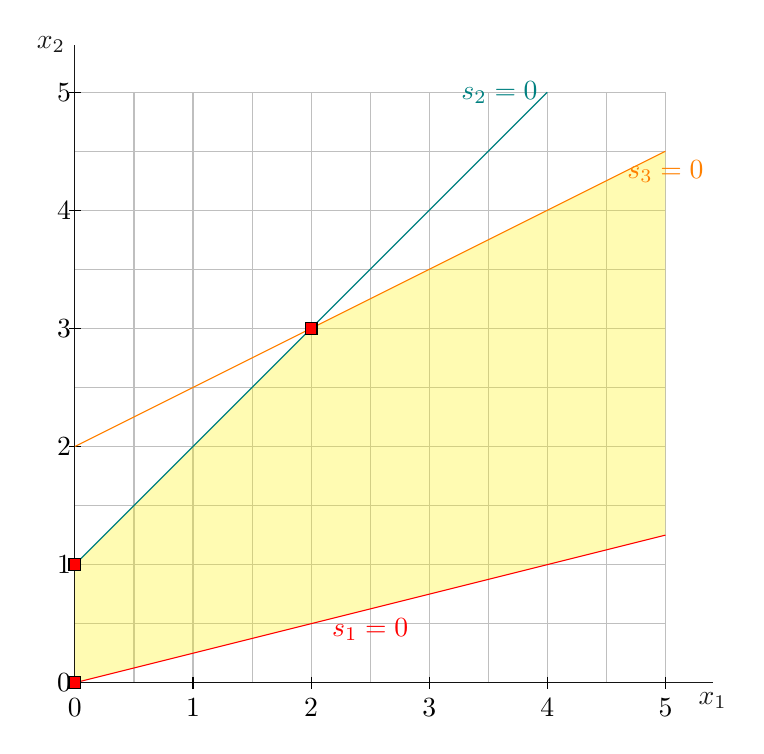
\begin{tikzpicture} [scale=1.5]
    \draw[gray!50, thin, step=.5] (0,0) grid (5,5);
    \draw[opacity=0.9] (0,0) -- (5.4,0) node[below] {$x_1$};
    \draw[opacity=0.9] (0,0) -- (0,5.4) node[left] {$x_2$}; % option \draw[very thick,->]

    \foreach \x in {0,...,5} \draw (\x,0.05) -- (\x,-0.05) node[below] {\x};
    \foreach \y in {0,...,5} \draw (-0.05,\y) -- (0.05,\y) node[left] {\y};

    \fill[yellow,opacity=0.3] (0,0) -- (0,1) -- (2,3) -- (5,4.5) --(5,1.25)-- cycle;

    \draw [red](0,0) -- node[below] {$s_1=0$} (5, 1.25);
    \draw [teal] (0,1)  --  (4,5) node[left, sloped] {$s_2=0$};
    \draw [orange](0,2) --  (5,4.5) node[below, sloped] {$s_3=0$}; %node[above right ,sloped] 
	\filldraw[fill=red] (-0.05,-0.05) rectangle (0.05,0.05);
	\filldraw[fill=red] (-0.05,.95) rectangle (0.05,1.05);
	\filldraw[fill=red] (1.95,2.95) rectangle (2.05,3.05);
\end{tikzpicture} \end{center} 
\end{minipage}

\begin{center}  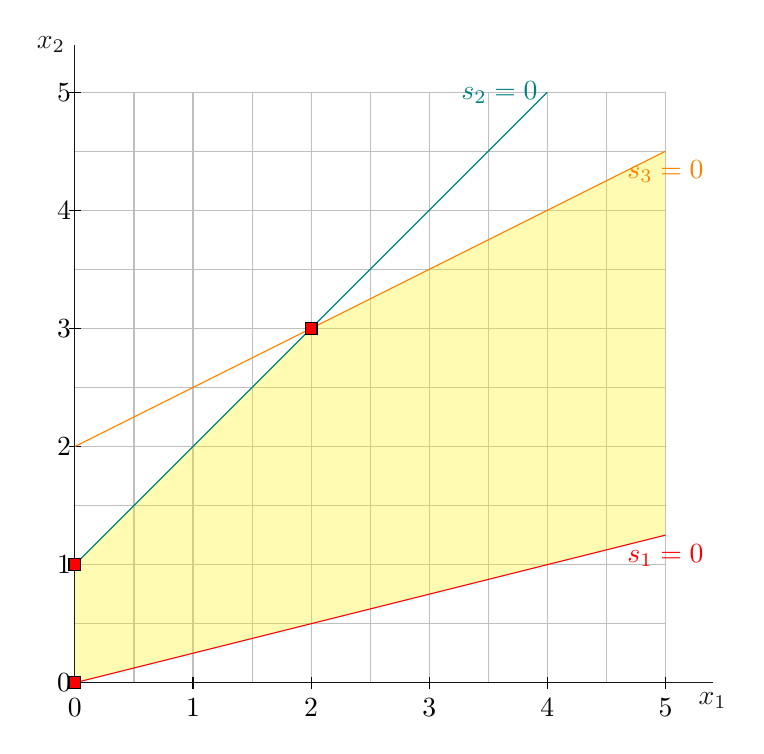
\begin{tikzpicture} [scale=1.5]
    \draw[gray!50, thin, step=.5] (0,0) grid (5,5);
    \draw[opacity=0.9] (0,0) -- (5.4,0) node[below] {$x_1$};
    \draw[opacity=0.9] (0,0) -- (0,5.4) node[left] {$x_2$}; % option \draw[very thick,->]

    \foreach \x in {0,...,5} \draw (\x,0.05) -- (\x,-0.05) node[below] {\x};
    \foreach \y in {0,...,5} \draw (-0.05,\y) -- (0.05,\y) node[left] {\y};

    \fill[yellow,opacity=0.3] (0,0) -- (0,1) -- (2,3) -- (5,4.5) --(5,1.25)-- cycle;

\draw[domain=0:4,smooth,variable=\x, teal] plot ({\x},{\x+1}) node[left] {$s_2=0$};
\draw[domain=0:5,smooth,variable=\x, red] plot ({\x},{\x*1/4}) node[below] {$s_1=0$};
%    \draw [red](0,0) -- node[below] {$s_1=0$} (5, 1.25);
    %\draw [teal] (0,1)  --  (4,5) node[left, sloped] {$s_2=0$};
    \draw [orange](0,2) --  (5,4.5) node[below, sloped] {$s_3=0$}; %node[above right ,sloped] 
	\filldraw[fill=red] (-0.05,-0.05) rectangle (0.05,0.05);
	\filldraw[fill=red] (-0.05,.95) rectangle (0.05,1.05);
	\filldraw[fill=red] (1.95,2.95) rectangle (2.05,3.05);
\end{tikzpicture} \end{center} 

% \draw[scale=0.5,domain=-3:3,smooth,variable=\x,blue] plot ({\x},{\x*\x});


\medskip E.g., consider the $s_3=0$ (orange) line, to find the extreme direction start at extreme point (2,3) and find another feasible point on the orange line, say (4,4) and subtract (2,3) from (4,4), which yields (2,1). 

\medskip This is related to the slope in two-dimensions, as discussed in class, the rise is 1 and the run is 2. So this direction has a slope of 1/2, but this does not carry over easily to higher dimensions where directions cannot be defined by a single number. 

\medskip To find the extreme directions we can change the right-hand-side to $\mathbf{b} = \mathbf{0}$, which forms a polyhedral cone (in yellow), and then add the constraint $x_1 + x_2 = 1$. The intersection of the cone and  $x_1 + x_2 = 1$ form a line segment.

\begin{minipage}[t][][b]{.4\linewidth} \vspace{0mm}
\begin{align*}
\mbox{max~~} & z = -5x_1 - x_2  \\
\mbox{s.t.~~} & x_1 - 4x_2 +s_1 = 0  \\
& -x_1 + x_2 + s_2 = 0 \\
& -x_1 + 2x_2 +s_3 = 0 \\
& x_1 + x_2 = 1 \\
& x_1, x_2, s_1, s_2, s_3 \ge 0.
\end{align*}
\end{minipage}%
\begin{minipage}[t][][b]{.6\linewidth}
\begin{center} 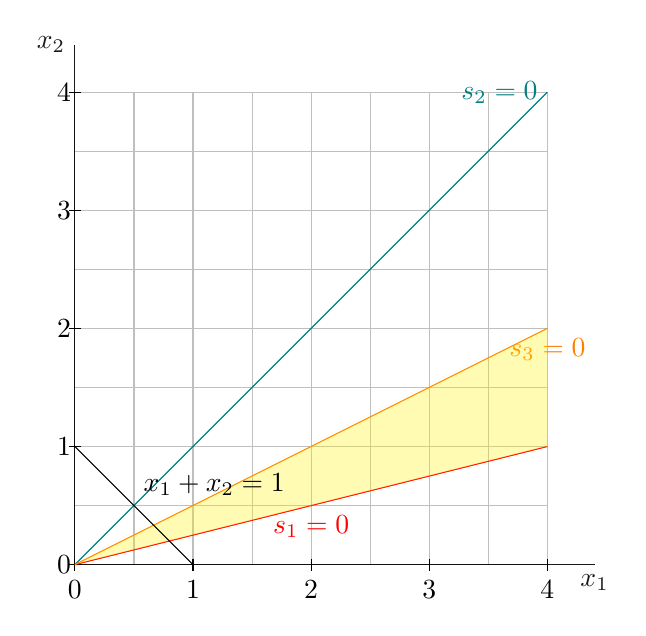
\begin{tikzpicture} [scale=1.5]
\draw[gray!50, thin, step=.5] (0,0) grid (4,4);
\draw[opacity=0.9] (0,0) -- (4.4,0) node[below] {$x_1$};
\draw[opacity=0.9] (0,0) -- (0,4.4) node[left] {$x_2$}; % option \draw[very thick,->]

\foreach \x in {0,...,4} \draw (\x,0.05) -- (\x,-0.05) node[below] {\x};
\foreach \y in {0,...,4} \draw (-0.05,\y) -- (0.05,\y) node[left] {\y};
        
\draw [red](0, 0) -- node[below] {$s_1=0$} (4, 1);
\draw [teal] (0,0)  -- (4,4) node[left, sloped] {$s_2=0$};
\draw [orange](0,0) -- (4,2) node[below, sloped] {$s_3=0$}; 
\fill[yellow,opacity=0.3] (0,0) -- (4,2) -- (4,1) --  cycle; % \draw [orange!50!blue] 

\draw [black] (0,1)  -- node[above right] {$x_1+x_2 = 1$} (1,0); 
\end{tikzpicture} \end{center} 
\end{minipage}



\begin{center} 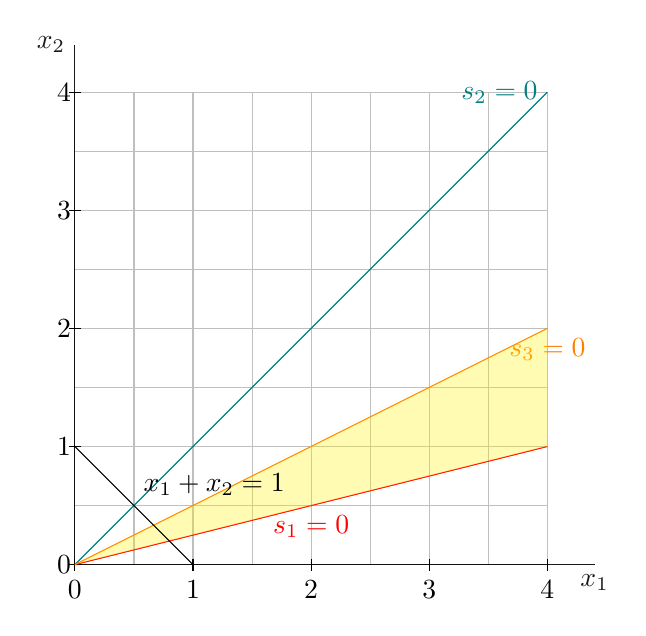
\begin{tikzpicture} [scale=1.5]
\draw[gray!50, thin, step=.5] (0,0) grid (4,4);
\draw[opacity=0.9] (0,0) -- (4.4,0) node[below] {$x_1$};
\draw[opacity=0.9] (0,0) -- (0,4.4) node[left] {$x_2$}; % option \draw[very thick,->]

\foreach \x in {0,...,4} \draw (\x,0.05) -- (\x,-0.05) node[below] {\x};
\foreach \y in {0,...,4} \draw (-0.05,\y) -- (0.05,\y) node[left] {\y};
        
\draw [red](0, 0) -- node[below] {$s_1=0$} (4, 1);
\draw [teal] (0,0)  -- (4,4) node[left, sloped] {$s_2=0$};
\draw [orange](0,0) -- (4,2) node[below, sloped] {$s_3=0$}; 
\fill[yellow,opacity=0.3] (0,0) -- (4,2) -- (4,1) --  cycle; % \draw [orange!50!blue] 

\draw [black] (0,1)  -- node[above right] {$x_1+x_2 = 1$} (1,0); 
\end{tikzpicture} \end{center} 


\medskip Magnifying for clarity, and removing the $s_2=0$ (teal) line, as it is redundant, and marking the extreme points of the new feasible region, (4/5, 1/5) and (2/3, 1/3), with red boxes, we have:

\begin{center}  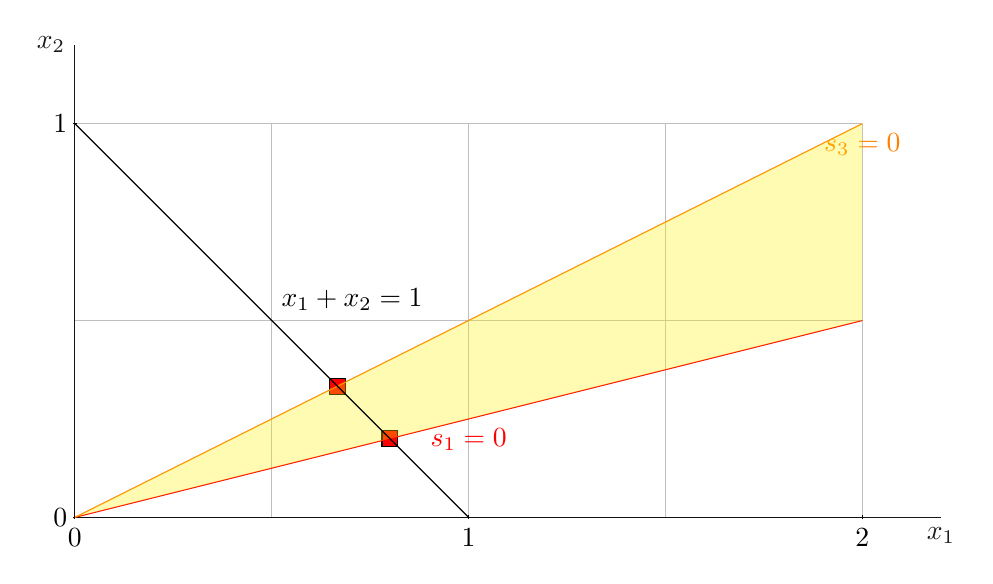
\begin{tikzpicture} [x=50mm, y=50mm] [scale=1.5]
\draw[gray!50, thin, step=.5] (0,0) grid (2,1);
\draw[opacity=0.9] (0,0) -- (2.2,0) node[below] {$x_1$};
\draw[opacity=0.9] (0,0) -- (0,1.2) node[left] {$x_2$}; % option \draw[very thick,->]

\foreach \x in {0,...,2} \draw (\x,0.005) -- (\x,-0.005) node[below] {\x};
\foreach \y in {0,...,1} \draw (-0.005,\y) -- (0.005,\y) node[left] {\y};

\filldraw[fill=red] (0.8-0.02,0.2-0.02) rectangle (0.8+0.02,0.2+0.02);
\filldraw[fill=red] (0.667-0.02,0.333-0.02) rectangle (0.667+0.02,0.333+0.02);

\draw [red](0, 0) -- node[below] {$s_1=0$} (2, .5);
\draw [orange](0,0) -- (2,1) node[below, sloped] {$s_3=0$}; 
\fill[yellow,opacity=0.3] (0,0) -- (2,.5) -- (2,1) --  cycle; % \draw [orange!50!blue] 
\draw [black] (0,1)  -- node[above right] {$x_1+x_2 = 1$} (1,0); 
\end{tikzpicture} \end{center} 

The extreme directions are thus (4/5, 1/5) and (2/3, 1/3). \\

{\bf Representation Theorem:} Let  $\mathbf{x_1}, \mathbf{x_2},\cdots \mathbf{x_k}$ be the set of extreme points of $\mathcal{S}$, and if $\mathcal{S}$ is unbounded, $\mathbf{d_1}, \mathbf{d_2},\cdots \mathbf{d_l}$ be the set of extreme directions. Then any $\mathbf{x} \in \mathcal{S}$ is equal to a convex combination of the extreme points and a non-negative linear combination of the extreme directions: $\mathbf{x} = \sum_{j=1}^k \lambda_j \mathbf{x_j} + \sum_{j=1}^l \mu_j \mathbf{d_j}$, where $\sum_{j=1}^k \lambda_j = 1$, $\lambda_j \ge 0,~\forall  j=1,2,\cdots,k$, and $\mu_j \ge 0,~\forall j=1,2,\cdots,l$.

 \begin{minipage}[t][][b]{.4\linewidth}
\begin{align*}
\mbox{max~~} & z = -5x_1 - x_2  \\\
\mbox{s.t.~~} & x_1 - 4x_2 +s_1 = 0  \\
& -x_1 + x_2 + s_2 = 1 \\
& -x_1 + 2x_2 +s_3 = 4 \\
& x_1, x_2, s_1, s_2, s_3 \ge 0.
\end{align*}
\end{minipage}%
\begin{minipage}[t][][b]{.6\linewidth}
\begin{center}  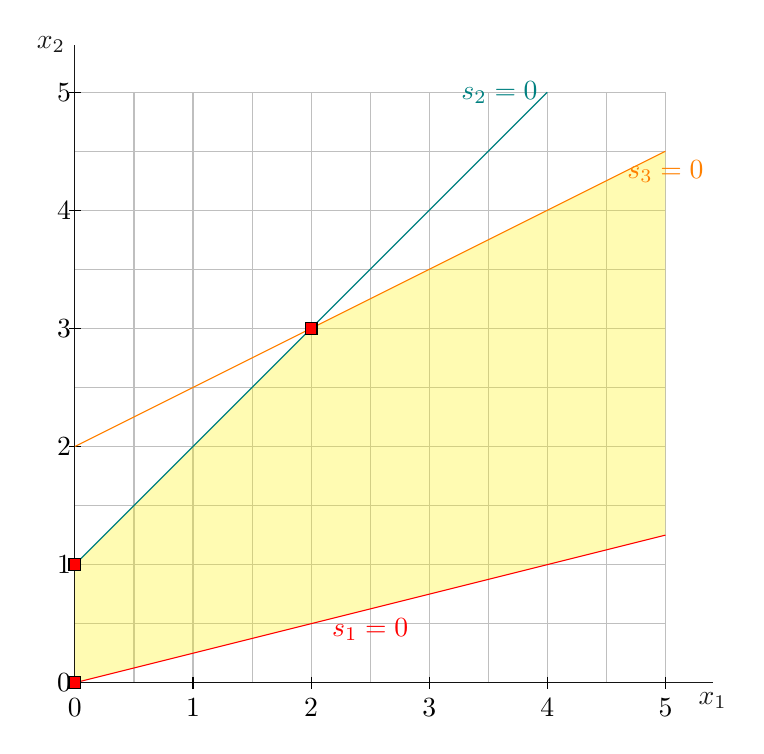
\begin{tikzpicture} [scale=1.5]
    \draw[gray!50, thin, step=.5] (0,0) grid (5,5);
    \draw[opacity=0.9] (0,0) -- (5.4,0) node[below] {$x_1$};
    \draw[opacity=0.9] (0,0) -- (0,5.4) node[left] {$x_2$}; % option \draw[very thick,->]

    \foreach \x in {0,...,5} \draw (\x,0.05) -- (\x,-0.05) node[below] {\x};
    \foreach \y in {0,...,5} \draw (-0.05,\y) -- (0.05,\y) node[left] {\y};

    \fill[yellow,opacity=0.3] (0,0) -- (0,1) -- (2,3) -- (5,4.5) --(5,1.25)-- cycle;

    \draw [red](0,0) -- node[below] {$s_1=0$} (5, 1.25);
    \draw [teal] (0,1)  --  (4,5) node[left, sloped] {$s_2=0$};
    \draw [orange](0,2) --  (5,4.5) node[below, sloped] {$s_3=0$}; %node[above right ,sloped] 
	\filldraw[fill=red] (-0.05,-0.05) rectangle (0.05,0.05);
	\filldraw[fill=red] (-0.05,.95) rectangle (0.05,1.05);
	\filldraw[fill=red] (1.95,2.95) rectangle (2.05,3.05);
\end{tikzpicture} \end{center} 
\end{minipage}

Represent point (1/2, 1) as a convex combination of the extreme points of the above LP.  Find $\lambda$s to solve the following system of equations:

$$\lambda_1 \left[
  \begin{array}{c}
  0 \\
  0 \\
  \end{array} \right]+
 \lambda_2 \left[
  \begin{array}{c}
  0 \\
  1 \\
  \end{array} \right] +
 \lambda_3 \left[
  \begin{array}{c}
  2 \\
  3 \\
  \end{array} \right]  =
 \left[
  \begin{array}{c}
  1/2 \\
  1 \\
  \end{array} \right] 
$$



